\documentclass[1p]{elsarticle_modified}
%\bibliographystyle{elsarticle-num}

%\usepackage[colorlinks]{hyperref}
%\usepackage{abbrmath_seonhwa} %\Abb, \Ascr, \Acal ,\Abf, \Afrak
\usepackage{amsfonts}
\usepackage{amssymb}
\usepackage{amsmath}
\usepackage{amsthm}
\usepackage{scalefnt}
\usepackage{amsbsy}
\usepackage{kotex}
\usepackage{caption}
\usepackage{subfig}
\usepackage{color}
\usepackage{graphicx}
\usepackage{xcolor} %% white, black, red, green, blue, cyan, magenta, yellow
\usepackage{float}
\usepackage{setspace}
\usepackage{hyperref}

\usepackage{tikz}
\usetikzlibrary{arrows}

\usepackage{multirow}
\usepackage{array} % fixed length table
\usepackage{hhline}

%%%%%%%%%%%%%%%%%%%%%
\makeatletter
\renewcommand*\env@matrix[1][\arraystretch]{%
	\edef\arraystretch{#1}%
	\hskip -\arraycolsep
	\let\@ifnextchar\new@ifnextchar
	\array{*\c@MaxMatrixCols c}}
\makeatother %https://tex.stackexchange.com/questions/14071/how-can-i-increase-the-line-spacing-in-a-matrix
%%%%%%%%%%%%%%%

\usepackage[normalem]{ulem}

\newcommand{\msout}[1]{\ifmmode\text{\sout{\ensuremath{#1}}}\else\sout{#1}\fi}
%SOURCE: \msout is \stkout macro in https://tex.stackexchange.com/questions/20609/strikeout-in-math-mode

\newcommand{\cancel}[1]{
	\ifmmode
	{\color{red}\msout{#1}}
	\else
	{\color{red}\sout{#1}}
	\fi
}

\newcommand{\add}[1]{
	{\color{blue}\uwave{#1}}
}

\newcommand{\replace}[2]{
	\ifmmode
	{\color{red}\msout{#1}}{\color{blue}\uwave{#2}}
	\else
	{\color{red}\sout{#1}}{\color{blue}\uwave{#2}}
	\fi
}

\newcommand{\Sol}{\mathcal{S}} %segment
\newcommand{\D}{D} %diagram
\newcommand{\A}{\mathcal{A}} %arc


%%%%%%%%%%%%%%%%%%%%%%%%%%%%%5 test

\def\sl{\operatorname{\textup{SL}}(2,\Cbb)}
\def\psl{\operatorname{\textup{PSL}}(2,\Cbb)}
\def\quan{\mkern 1mu \triangleright \mkern 1mu}

\theoremstyle{definition}
\newtheorem{thm}{Theorem}[section]
\newtheorem{prop}[thm]{Proposition}
\newtheorem{lem}[thm]{Lemma}
\newtheorem{ques}[thm]{Question}
\newtheorem{cor}[thm]{Corollary}
\newtheorem{defn}[thm]{Definition}
\newtheorem{exam}[thm]{Example}
\newtheorem{rmk}[thm]{Remark}
\newtheorem{alg}[thm]{Algorithm}

\newcommand{\I}{\sqrt{-1}}
\begin{document}

%\begin{frontmatter}
%
%\title{Boundary parabolic representations of knots up to 8 crossings}
%
%%% Group authors per affiliation:
%\author{Yunhi Cho} 
%\address{Department of Mathematics, University of Seoul, Seoul, Korea}
%\ead{yhcho@uos.ac.kr}
%
%
%\author{Seonhwa Kim} %\fnref{s_kim}}
%\address{Center for Geometry and Physics, Institute for Basic Science, Pohang, 37673, Korea}
%\ead{ryeona17@ibs.re.kr}
%
%\author{Hyuk Kim}
%\address{Department of Mathematical Sciences, Seoul National University, Seoul 08826, Korea}
%\ead{hyukkim@snu.ac.kr}
%
%\author{Seokbeom Yoon}
%\address{Department of Mathematical Sciences, Seoul National University, Seoul, 08826,  Korea}
%\ead{sbyoon15@snu.ac.kr}
%
%\begin{abstract}
%We find all boundary parabolic representation of knots up to 8 crossings.
%
%\end{abstract}
%\begin{keyword}
%    \MSC[2010] 57M25 
%\end{keyword}
%
%\end{frontmatter}

%\linenumbers
%\tableofcontents
%
\newcommand\colored[1]{\textcolor{white}{\rule[-0.35ex]{0.8em}{1.4ex}}\kern-0.8em\color{red} #1}%
%\newcommand\colored[1]{\textcolor{white}{ #1}\kern-2.17ex	\textcolor{white}{ #1}\kern-1.81ex	\textcolor{white}{ #1}\kern-2.15ex\color{red}#1	}

{\Large $\underline{12a_{0937}~(K12a_{0937})}$}

\setlength{\tabcolsep}{10pt}
\renewcommand{\arraystretch}{1.6}
\vspace{1cm}\begin{tabular}{m{100pt}>{\centering\arraybackslash}m{274pt}}
\multirow{5}{120pt}{
	\centering
	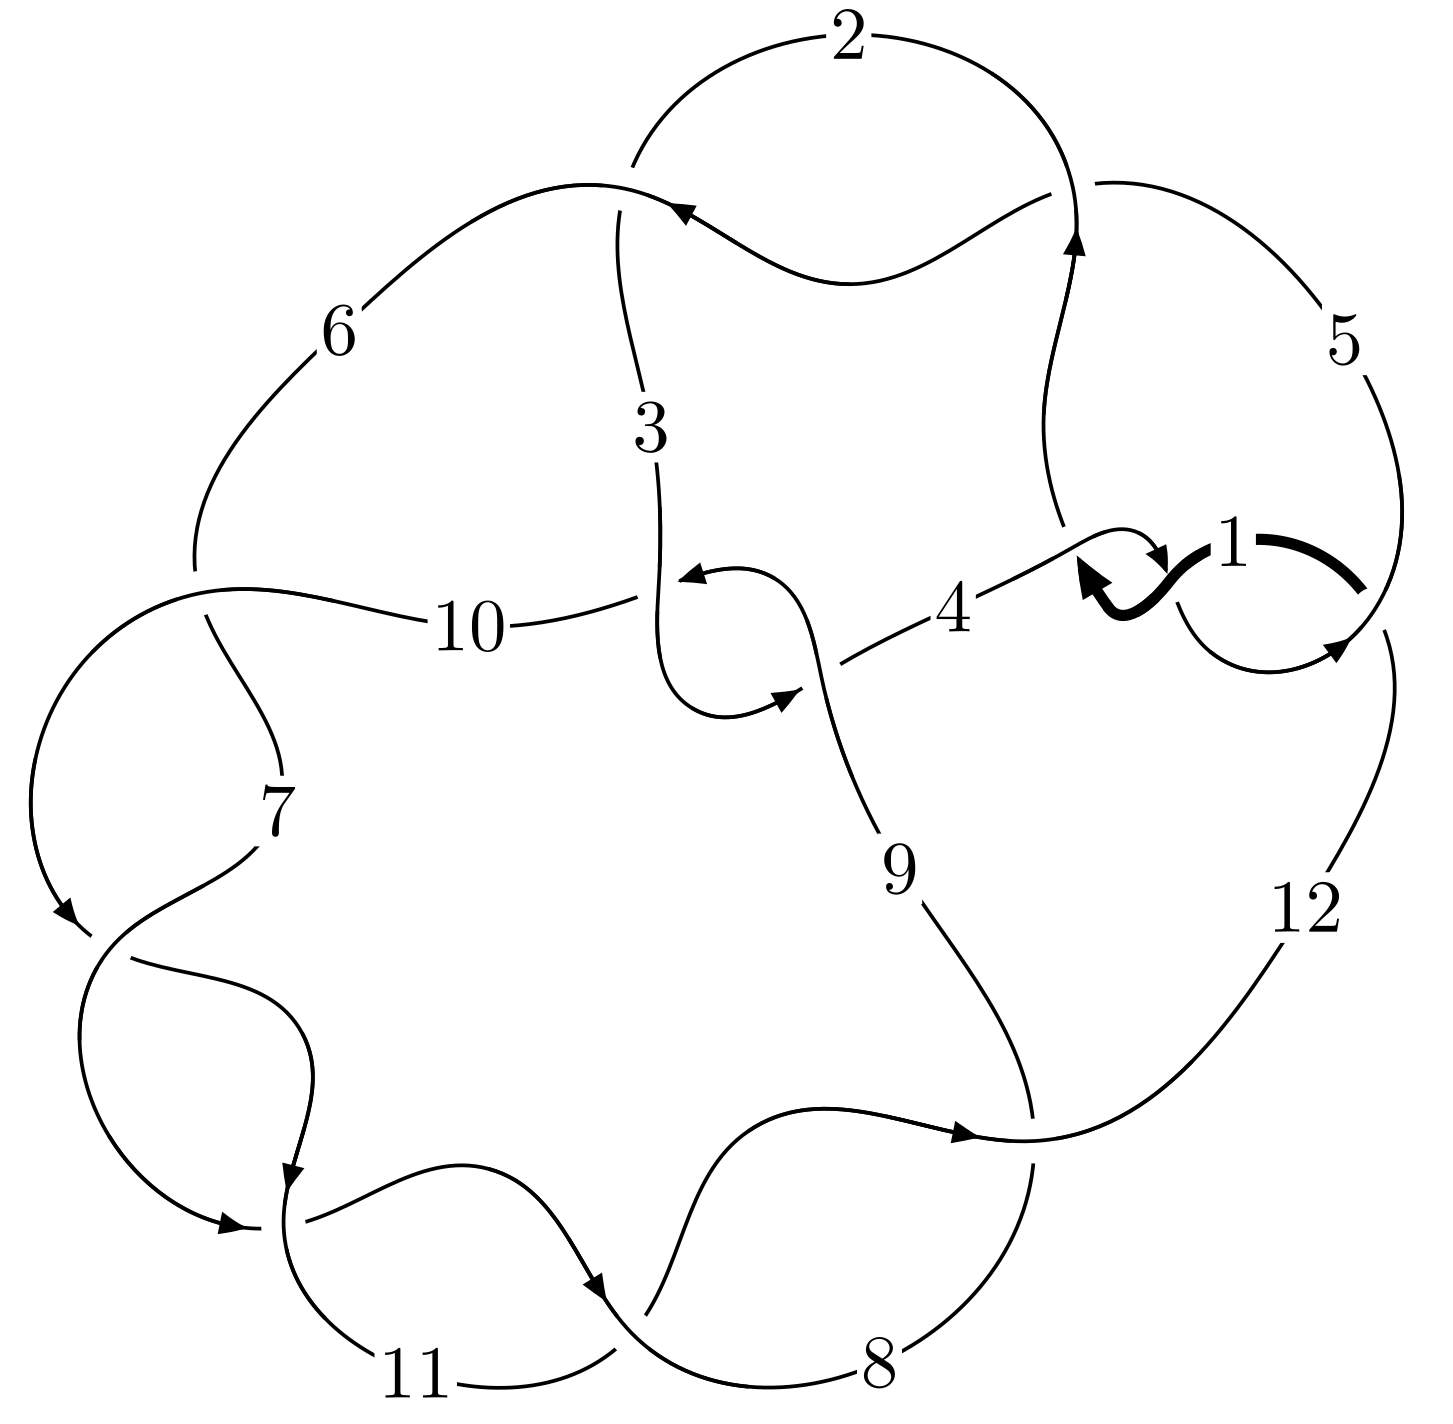
\includegraphics[width=112pt]{../../../GIT/diagram.site/Diagrams/png/1738_12a_0937.png}\\
\ \ \ A knot diagram\footnotemark}&
\allowdisplaybreaks
\textbf{Linearized knot diagam} \\
\cline{2-2}
 &
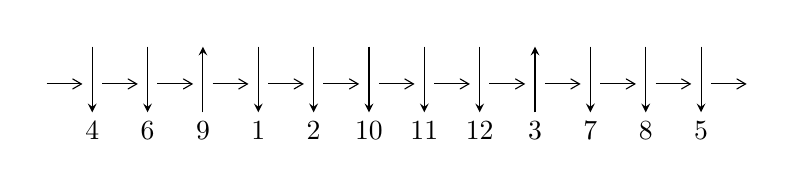
\begin{tikzpicture}[x=20pt, y=17pt]
	% nodes
	\node (C0) at (0, 0) {};
	\node (C1) at (1, 0) {};
	\node (C1U) at (1, +1) {};
	\node (C1D) at (1, -1) {4};

	\node (C2) at (2, 0) {};
	\node (C2U) at (2, +1) {};
	\node (C2D) at (2, -1) {6};

	\node (C3) at (3, 0) {};
	\node (C3U) at (3, +1) {};
	\node (C3D) at (3, -1) {9};

	\node (C4) at (4, 0) {};
	\node (C4U) at (4, +1) {};
	\node (C4D) at (4, -1) {1};

	\node (C5) at (5, 0) {};
	\node (C5U) at (5, +1) {};
	\node (C5D) at (5, -1) {2};

	\node (C6) at (6, 0) {};
	\node (C6U) at (6, +1) {};
	\node (C6D) at (6, -1) {10};

	\node (C7) at (7, 0) {};
	\node (C7U) at (7, +1) {};
	\node (C7D) at (7, -1) {11};

	\node (C8) at (8, 0) {};
	\node (C8U) at (8, +1) {};
	\node (C8D) at (8, -1) {12};

	\node (C9) at (9, 0) {};
	\node (C9U) at (9, +1) {};
	\node (C9D) at (9, -1) {3};

	\node (C10) at (10, 0) {};
	\node (C10U) at (10, +1) {};
	\node (C10D) at (10, -1) {7};

	\node (C11) at (11, 0) {};
	\node (C11U) at (11, +1) {};
	\node (C11D) at (11, -1) {8};

	\node (C12) at (12, 0) {};
	\node (C12U) at (12, +1) {};
	\node (C12D) at (12, -1) {5};
	\node (C13) at (13, 0) {};

	% arrows
	\draw[->,>={angle 60}]
	(C0) edge (C1) (C1) edge (C2) (C2) edge (C3) (C3) edge (C4) (C4) edge (C5) (C5) edge (C6) (C6) edge (C7) (C7) edge (C8) (C8) edge (C9) (C9) edge (C10) (C10) edge (C11) (C11) edge (C12) (C12) edge (C13) ;	\draw[->,>=stealth]
	(C1U) edge (C1D) (C2U) edge (C2D) (C3D) edge (C3U) (C4U) edge (C4D) (C5U) edge (C5D) (C6U) edge (C6D) (C7U) edge (C7D) (C8U) edge (C8D) (C9D) edge (C9U) (C10U) edge (C10D) (C11U) edge (C11D) (C12U) edge (C12D) ;
	\end{tikzpicture} \\
\hhline{~~} \\& 
\textbf{Solving Sequence} \\ \cline{2-2} 
 &
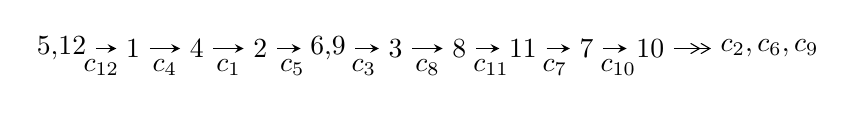
\begin{tikzpicture}[x=23pt, y=7pt]
	% node
	\node (A0) at (-1/8, 0) {5,12};
	\node (A1) at (1, 0) {1};
	\node (A2) at (2, 0) {4};
	\node (A3) at (3, 0) {2};
	\node (A4) at (65/16, 0) {6,9};
	\node (A5) at (41/8, 0) {3};
	\node (A6) at (49/8, 0) {8};
	\node (A7) at (57/8, 0) {11};
	\node (A8) at (65/8, 0) {7};
	\node (A9) at (73/8, 0) {10};
	\node (C1) at (1/2, -1) {$c_{12}$};
	\node (C2) at (3/2, -1) {$c_{4}$};
	\node (C3) at (5/2, -1) {$c_{1}$};
	\node (C4) at (7/2, -1) {$c_{5}$};
	\node (C5) at (37/8, -1) {$c_{3}$};
	\node (C6) at (45/8, -1) {$c_{8}$};
	\node (C7) at (53/8, -1) {$c_{11}$};
	\node (C8) at (61/8, -1) {$c_{7}$};
	\node (C9) at (69/8, -1) {$c_{10}$};
	\node (A10) at (11, 0) {$c_{2},c_{6},c_{9}$};

	% edge
	\draw[->,>=stealth]	
	(A0) edge (A1) (A1) edge (A2) (A2) edge (A3) (A3) edge (A4) (A4) edge (A5) (A5) edge (A6) (A6) edge (A7) (A7) edge (A8) (A8) edge (A9) ;
	\draw[->>,>={angle 60}]	
	(A9) edge (A10);
\end{tikzpicture} \\ 

\end{tabular} \\

\footnotetext{
The image of knot diagram is generated by the software ``\textbf{Draw programme}" developed by Andrew Bartholomew(\url{http://www.layer8.co.uk/maths/draw/index.htm\#Running-draw}), where we modified some parts for our purpose(\url{https://github.com/CATsTAILs/LinksPainter}).
}\phantom \\ \newline 
\centering \textbf{Ideals for irreducible components\footnotemark of $X_{\text{par}}$} 
 
\begin{align*}
I^u_{1}&=\langle 
u^{44}+4 u^{43}+\cdots+2 b+1,\;-4 u^{44}-14 u^{43}+\cdots+2 a+11,\;u^{45}+3 u^{44}+\cdots-4 u-1\rangle \\
I^u_{2}&=\langle 
- u^2 a+b- a,\;- u^2 a+a^2+a u- a- u,\;u^3- u^2+2 u-1\rangle \\
\\
\end{align*}
\raggedright * 2 irreducible components of $\dim_{\mathbb{C}}=0$, with total 51 representations.\\
\footnotetext{All coefficients of polynomials are rational numbers. But the coefficients are sometimes approximated in decimal forms when there is not enough margin.}
\newpage
\renewcommand{\arraystretch}{1}
\centering \section*{I. $I^u_{1}= \langle u^{44}+4 u^{43}+\cdots+2 b+1,\;-4 u^{44}-14 u^{43}+\cdots+2 a+11,\;u^{45}+3 u^{44}+\cdots-4 u-1 \rangle$}
\flushleft \textbf{(i) Arc colorings}\\
\begin{tabular}{m{7pt} m{180pt} m{7pt} m{180pt} }
\flushright $a_{5}=$&$\begin{pmatrix}0\\u\end{pmatrix}$ \\
\flushright $a_{12}=$&$\begin{pmatrix}1\\0\end{pmatrix}$ \\
\flushright $a_{1}=$&$\begin{pmatrix}1\\u^2\end{pmatrix}$ \\
\flushright $a_{4}=$&$\begin{pmatrix}u\\u^3+u\end{pmatrix}$ \\
\flushright $a_{2}=$&$\begin{pmatrix}u^2+1\\u^4+2 u^2\end{pmatrix}$ \\
\flushright $a_{6}=$&$\begin{pmatrix}- u^5-2 u^3- u\\- u^7-3 u^5-2 u^3+u\end{pmatrix}$ \\
\flushright $a_{9}=$&$\begin{pmatrix}2 u^{44}+7 u^{43}+\cdots-2 u-\frac{11}{2}\\-\frac{1}{2} u^{44}-2 u^{43}+\cdots+3 u-\frac{1}{2}\end{pmatrix}$ \\
\flushright $a_{3}=$&$\begin{pmatrix}- u^8-3 u^6-3 u^4+1\\- u^{10}-4 u^8-5 u^6+3 u^2\end{pmatrix}$ \\
\flushright $a_{8}=$&$\begin{pmatrix}\frac{3}{2} u^{44}+5 u^{43}+\cdots+u-6\\-\frac{1}{2} u^{44}-2 u^{43}+\cdots+3 u-\frac{1}{2}\end{pmatrix}$ \\
\flushright $a_{11}=$&$\begin{pmatrix}-\frac{1}{2} u^{44}- u^{43}+\cdots+7 u+1\\-\frac{1}{2} u^{44}- u^{43}+\cdots+2 u+\frac{1}{2}\end{pmatrix}$ \\
\flushright $a_{7}=$&$\begin{pmatrix}-\frac{1}{2} u^{42}- u^{41}+\cdots+7 u-\frac{1}{2}\\-\frac{1}{2} u^{44}- u^{43}+\cdots+u+\frac{1}{2}\end{pmatrix}$ \\
\flushright $a_{10}=$&$\begin{pmatrix}- u^{44}- u^{43}+\cdots+7 u-\frac{7}{2}\\-\frac{3}{2} u^{44}-5 u^{43}+\cdots+7 u+\frac{1}{2}\end{pmatrix}$\\&\end{tabular}
\flushleft \textbf{(ii) Obstruction class $= -1$}\\~\\
\flushleft \textbf{(iii) Cusp Shapes $= u^{44}+\frac{5}{2} u^{43}+\cdots-\frac{15}{2} u-\frac{21}{2}$}\\~\\
\newpage\renewcommand{\arraystretch}{1}
\flushleft \textbf{(iv) u-Polynomials at the component}\newline \\
\begin{tabular}{m{50pt}|m{274pt}}
Crossings & \hspace{64pt}u-Polynomials at each crossing \\
\hline $$\begin{aligned}c_{1},c_{4},c_{12}\end{aligned}$$&$\begin{aligned}
&u^{45}-3 u^{44}+\cdots-4 u+1
\end{aligned}$\\
\hline $$\begin{aligned}c_{2},c_{5}\end{aligned}$$&$\begin{aligned}
&u^{45}+3 u^{44}+\cdots-2 u+41
\end{aligned}$\\
\hline $$\begin{aligned}c_{3},c_{9}\end{aligned}$$&$\begin{aligned}
&u^{45}- u^{44}+\cdots-32 u+64
\end{aligned}$\\
\hline $$\begin{aligned}c_{6},c_{7},c_{8}\\c_{10},c_{11}\end{aligned}$$&$\begin{aligned}
&u^{45}+4 u^{44}+\cdots+u-1
\end{aligned}$\\
\hline
\end{tabular}\\~\\
\newpage\renewcommand{\arraystretch}{1}
\flushleft \textbf{(v) Riley Polynomials at the component}\newline \\
\begin{tabular}{m{50pt}|m{274pt}}
Crossings & \hspace{64pt}Riley Polynomials at each crossing \\
\hline $$\begin{aligned}c_{1},c_{4},c_{12}\end{aligned}$$&$\begin{aligned}
&y^{45}+37 y^{44}+\cdots+40 y-1
\end{aligned}$\\
\hline $$\begin{aligned}c_{2},c_{5}\end{aligned}$$&$\begin{aligned}
&y^{45}-39 y^{44}+\cdots+54616 y-1681
\end{aligned}$\\
\hline $$\begin{aligned}c_{3},c_{9}\end{aligned}$$&$\begin{aligned}
&y^{45}+35 y^{44}+\cdots+29696 y-4096
\end{aligned}$\\
\hline $$\begin{aligned}c_{6},c_{7},c_{8}\\c_{10},c_{11}\end{aligned}$$&$\begin{aligned}
&y^{45}-62 y^{44}+\cdots+33 y-1
\end{aligned}$\\
\hline
\end{tabular}\\~\\
\newpage\flushleft \textbf{(vi) Complex Volumes and Cusp Shapes}
$$\begin{array}{c|c|c}  
\text{Solutions to }I^u_{1}& \I (\text{vol} + \sqrt{-1}CS) & \text{Cusp shape}\\
 \hline 
\begin{aligned}
u &= -0.890413 + 0.122697 I \\
a &= -1.10889 - 1.11126 I \\
b &= -1.76542 + 0.09202 I\end{aligned}
 & \phantom{-}18.6493 + 7.3520 I & -17.3944 - 3.6030 I \\ \hline\begin{aligned}
u &= -0.890413 - 0.122697 I \\
a &= -1.10889 + 1.11126 I \\
b &= -1.76542 - 0.09202 I\end{aligned}
 & \phantom{-}18.6493 - 7.3520 I & -17.3944 + 3.6030 I \\ \hline\begin{aligned}
u &= -0.857781 + 0.085739 I \\
a &= \phantom{-}0.773971 + 0.850892 I \\
b &= \phantom{-}1.146650 - 0.350828 I\end{aligned}
 & -10.38620 + 5.44992 I & -17.1451 - 4.4258 I \\ \hline\begin{aligned}
u &= -0.857781 - 0.085739 I \\
a &= \phantom{-}0.773971 - 0.850892 I \\
b &= \phantom{-}1.146650 + 0.350828 I\end{aligned}
 & -10.38620 - 5.44992 I & -17.1451 + 4.4258 I \\ \hline\begin{aligned}
u &= \phantom{-}0.851384\phantom{ +0.000000I} \\
a &= \phantom{-}1.98833\phantom{ +0.000000I} \\
b &= \phantom{-}1.74823\phantom{ +0.000000I}\end{aligned}
 & -15.7842\phantom{ +0.000000I} & -16.5970\phantom{ +0.000000I} \\ \hline\begin{aligned}
u &= -0.826935 + 0.030025 I \\
a &= -0.276934 - 0.575320 I \\
b &= -0.381901 + 0.636194 I\end{aligned}
 & -5.58348 + 2.07140 I & -14.3541 - 3.3642 I \\ \hline\begin{aligned}
u &= -0.826935 - 0.030025 I \\
a &= -0.276934 + 0.575320 I \\
b &= -0.381901 - 0.636194 I\end{aligned}
 & -5.58348 - 2.07140 I & -14.3541 + 3.3642 I \\ \hline\begin{aligned}
u &= \phantom{-}0.606365 + 0.531100 I \\
a &= \phantom{-}0.104984 + 1.236330 I \\
b &= -1.74792 - 0.01574 I\end{aligned}
 & -14.7030 - 2.1539 I & -15.6545 + 3.1266 I \\ \hline\begin{aligned}
u &= \phantom{-}0.606365 - 0.531100 I \\
a &= \phantom{-}0.104984 - 1.236330 I \\
b &= -1.74792 + 0.01574 I\end{aligned}
 & -14.7030 + 2.1539 I & -15.6545 - 3.1266 I \\ \hline\begin{aligned}
u &= \phantom{-}0.778750\phantom{ +0.000000I} \\
a &= -1.54037\phantom{ +0.000000I} \\
b &= -1.06860\phantom{ +0.000000I}\end{aligned}
 & -5.57462\phantom{ +0.000000I} & -16.4290\phantom{ +0.000000I}\\
 \hline 
 \end{array}$$\newpage$$\begin{array}{c|c|c}  
\text{Solutions to }I^u_{1}& \I (\text{vol} + \sqrt{-1}CS) & \text{Cusp shape}\\
 \hline 
\begin{aligned}
u &= -0.110795 + 1.218650 I \\
a &= -1.31939 + 1.71047 I \\
b &= \phantom{-}1.61924 - 0.05616 I\end{aligned}
 & -5.93702 + 1.70967 I & -11.27232 + 1.90310 I \\ \hline\begin{aligned}
u &= -0.110795 - 1.218650 I \\
a &= -1.31939 - 1.71047 I \\
b &= \phantom{-}1.61924 + 0.05616 I\end{aligned}
 & -5.93702 - 1.70967 I & -11.27232 - 1.90310 I \\ \hline\begin{aligned}
u &= -0.002801 + 1.227720 I \\
a &= \phantom{-}0.43866 - 1.57194 I \\
b &= -0.738328 + 0.291820 I\end{aligned}
 & \phantom{-}2.19010 + 0.49707 I & -9.03459 - 1.32514 I \\ \hline\begin{aligned}
u &= -0.002801 - 1.227720 I \\
a &= \phantom{-}0.43866 + 1.57194 I \\
b &= -0.738328 - 0.291820 I\end{aligned}
 & \phantom{-}2.19010 - 0.49707 I & -9.03459 + 1.32514 I \\ \hline\begin{aligned}
u &= -0.463428 + 1.150540 I \\
a &= \phantom{-}0.206323 - 0.367607 I \\
b &= -1.77236 - 0.07475 I\end{aligned}
 & -17.6778 - 2.5277 I & -14.7181 + 0. I\phantom{ +0.000000I} \\ \hline\begin{aligned}
u &= -0.463428 - 1.150540 I \\
a &= \phantom{-}0.206323 + 0.367607 I \\
b &= -1.77236 + 0.07475 I\end{aligned}
 & -17.6778 + 2.5277 I & -14.7181 + 0. I\phantom{ +0.000000I} \\ \hline\begin{aligned}
u &= -0.407555 + 1.183180 I \\
a &= -0.449308 - 0.082403 I \\
b &= \phantom{-}1.184170 + 0.302548 I\end{aligned}
 & -7.01503 - 0.90790 I & -14.2280 + 0. I\phantom{ +0.000000I} \\ \hline\begin{aligned}
u &= -0.407555 - 1.183180 I \\
a &= -0.449308 + 0.082403 I \\
b &= \phantom{-}1.184170 - 0.302548 I\end{aligned}
 & -7.01503 + 0.90790 I & -14.2280 + 0. I\phantom{ +0.000000I} \\ \hline\begin{aligned}
u &= -0.370756 + 1.245550 I \\
a &= \phantom{-}0.615468 + 0.827180 I \\
b &= -0.445891 - 0.613389 I\end{aligned}
 & -1.82707 + 2.23489 I & \phantom{-0.000000 } 0 \\ \hline\begin{aligned}
u &= -0.370756 - 1.245550 I \\
a &= \phantom{-}0.615468 - 0.827180 I \\
b &= -0.445891 + 0.613389 I\end{aligned}
 & -1.82707 - 2.23489 I & \phantom{-0.000000 } 0\\
 \hline 
 \end{array}$$\newpage$$\begin{array}{c|c|c}  
\text{Solutions to }I^u_{1}& \I (\text{vol} + \sqrt{-1}CS) & \text{Cusp shape}\\
 \hline 
\begin{aligned}
u &= \phantom{-}0.085876 + 1.300140 I \\
a &= \phantom{-}0.31567 + 1.38001 I \\
b &= -0.051237 - 0.435616 I\end{aligned}
 & \phantom{-}4.23150 - 2.03860 I & \phantom{-0.000000 } 0 \\ \hline\begin{aligned}
u &= \phantom{-}0.085876 - 1.300140 I \\
a &= \phantom{-}0.31567 - 1.38001 I \\
b &= -0.051237 + 0.435616 I\end{aligned}
 & \phantom{-}4.23150 + 2.03860 I & \phantom{-0.000000 } 0 \\ \hline\begin{aligned}
u &= \phantom{-}0.334888 + 1.264580 I \\
a &= -0.392426 + 1.134500 I \\
b &= -1.068570 - 0.086970 I\end{aligned}
 & -1.65436 - 4.01424 I & \phantom{-0.000000 } 0 \\ \hline\begin{aligned}
u &= \phantom{-}0.334888 - 1.264580 I \\
a &= -0.392426 - 1.134500 I \\
b &= -1.068570 + 0.086970 I\end{aligned}
 & -1.65436 + 4.01424 I & \phantom{-0.000000 } 0 \\ \hline\begin{aligned}
u &= \phantom{-}0.242153 + 1.287270 I \\
a &= \phantom{-}0.318641 - 0.571138 I \\
b &= \phantom{-}0.280859 + 0.154657 I\end{aligned}
 & \phantom{-}2.59980 - 3.13937 I & \phantom{-0.000000 } 0 \\ \hline\begin{aligned}
u &= \phantom{-}0.242153 - 1.287270 I \\
a &= \phantom{-}0.318641 + 0.571138 I \\
b &= \phantom{-}0.280859 - 0.154657 I\end{aligned}
 & \phantom{-}2.59980 + 3.13937 I & \phantom{-0.000000 } 0 \\ \hline\begin{aligned}
u &= \phantom{-}0.503331 + 0.451082 I \\
a &= -0.360474 - 1.020470 I \\
b &= \phantom{-}1.066120 + 0.076462 I\end{aligned}
 & -4.50790 - 1.79515 I & -15.5943 + 4.2867 I \\ \hline\begin{aligned}
u &= \phantom{-}0.503331 - 0.451082 I \\
a &= -0.360474 + 1.020470 I \\
b &= \phantom{-}1.066120 - 0.076462 I\end{aligned}
 & -4.50790 + 1.79515 I & -15.5943 - 4.2867 I \\ \hline\begin{aligned}
u &= \phantom{-}0.391513 + 1.271870 I \\
a &= \phantom{-}0.32209 - 1.48073 I \\
b &= \phantom{-}1.74641 + 0.02116 I\end{aligned}
 & -11.83510 - 4.45927 I & \phantom{-0.000000 } 0 \\ \hline\begin{aligned}
u &= \phantom{-}0.391513 - 1.271870 I \\
a &= \phantom{-}0.32209 + 1.48073 I \\
b &= \phantom{-}1.74641 - 0.02116 I\end{aligned}
 & -11.83510 + 4.45927 I & \phantom{-0.000000 } 0\\
 \hline 
 \end{array}$$\newpage$$\begin{array}{c|c|c}  
\text{Solutions to }I^u_{1}& \I (\text{vol} + \sqrt{-1}CS) & \text{Cusp shape}\\
 \hline 
\begin{aligned}
u &= -0.371472 + 1.293170 I \\
a &= -0.36103 - 1.45695 I \\
b &= -0.326465 + 0.656457 I\end{aligned}
 & -1.45817 + 6.38100 I & \phantom{-0.000000 } 0 \\ \hline\begin{aligned}
u &= -0.371472 - 1.293170 I \\
a &= -0.36103 + 1.45695 I \\
b &= -0.326465 - 0.656457 I\end{aligned}
 & -1.45817 - 6.38100 I & \phantom{-0.000000 } 0 \\ \hline\begin{aligned}
u &= \phantom{-}0.627430\phantom{ +0.000000I} \\
a &= \phantom{-}0.675315\phantom{ +0.000000I} \\
b &= \phantom{-}0.234560\phantom{ +0.000000I}\end{aligned}
 & -1.43225\phantom{ +0.000000I} & -5.16570\phantom{ +0.000000I} \\ \hline\begin{aligned}
u &= -0.385838 + 1.331430 I \\
a &= -0.13299 + 1.85543 I \\
b &= \phantom{-}1.112000 - 0.380680 I\end{aligned}
 & -5.94556 + 9.91745 I & \phantom{-0.000000 } 0 \\ \hline\begin{aligned}
u &= -0.385838 - 1.331430 I \\
a &= -0.13299 - 1.85543 I \\
b &= \phantom{-}1.112000 + 0.380680 I\end{aligned}
 & -5.94556 - 9.91745 I & \phantom{-0.000000 } 0 \\ \hline\begin{aligned}
u &= \phantom{-}0.145397 + 1.390720 I \\
a &= -1.28933 - 1.01084 I \\
b &= \phantom{-}0.939446 + 0.150253 I\end{aligned}
 & \phantom{-}1.30405 - 3.95914 I & \phantom{-0.000000 } 0 \\ \hline\begin{aligned}
u &= \phantom{-}0.145397 - 1.390720 I \\
a &= -1.28933 + 1.01084 I \\
b &= \phantom{-}0.939446 - 0.150253 I\end{aligned}
 & \phantom{-}1.30405 + 3.95914 I & \phantom{-0.000000 } 0 \\ \hline\begin{aligned}
u &= -0.39751 + 1.35949 I \\
a &= \phantom{-}0.53384 - 2.10202 I \\
b &= -1.75547 + 0.10280 I\end{aligned}
 & -16.1695 + 11.9726 I & \phantom{-0.000000 } 0 \\ \hline\begin{aligned}
u &= -0.39751 - 1.35949 I \\
a &= \phantom{-}0.53384 + 2.10202 I \\
b &= -1.75547 - 0.10280 I\end{aligned}
 & -16.1695 - 11.9726 I & \phantom{-0.000000 } 0 \\ \hline\begin{aligned}
u &= \phantom{-}0.15162 + 1.44483 I \\
a &= \phantom{-}1.95312 + 1.07952 I \\
b &= -1.72058 - 0.03402 I\end{aligned}
 & -8.28166 - 4.65852 I & \phantom{-0.000000 } 0\\
 \hline 
 \end{array}$$\newpage$$\begin{array}{c|c|c}  
\text{Solutions to }I^u_{1}& \I (\text{vol} + \sqrt{-1}CS) & \text{Cusp shape}\\
 \hline 
\begin{aligned}
u &= \phantom{-}0.15162 - 1.44483 I \\
a &= \phantom{-}1.95312 - 1.07952 I \\
b &= -1.72058 + 0.03402 I\end{aligned}
 & -8.28166 + 4.65852 I & \phantom{-0.000000 } 0 \\ \hline\begin{aligned}
u &= -0.369157\phantom{ +0.000000I} \\
a &= \phantom{-}2.62661\phantom{ +0.000000I} \\
b &= \phantom{-}1.63816\phantom{ +0.000000I}\end{aligned}
 & -9.52192\phantom{ +0.000000I} & -4.22190\phantom{ +0.000000I} \\ \hline\begin{aligned}
u &= \phantom{-}0.271798 + 0.224791 I \\
a &= \phantom{-}0.661349 + 1.168710 I \\
b &= -0.244731 - 0.245078 I\end{aligned}
 & -0.383394 - 0.784998 I & -9.02382 + 8.78053 I \\ \hline\begin{aligned}
u &= \phantom{-}0.271798 - 0.224791 I \\
a &= \phantom{-}0.661349 - 1.168710 I \\
b &= -0.244731 + 0.245078 I\end{aligned}
 & -0.383394 + 0.784998 I & -9.02382 - 8.78053 I \\ \hline\begin{aligned}
u &= -0.183739\phantom{ +0.000000I} \\
a &= -2.85656\phantom{ +0.000000I} \\
b &= -0.704396\phantom{ +0.000000I}\end{aligned}
 & -1.23322\phantom{ +0.000000I} & -6.78810\phantom{ +0.000000I}\\
 \hline 
 \end{array}$$\newpage\newpage\renewcommand{\arraystretch}{1}
\centering \section*{II. $I^u_{2}= \langle - u^2 a+b- a,\;- u^2 a+a^2+a u- a- u,\;u^3- u^2+2 u-1 \rangle$}
\flushleft \textbf{(i) Arc colorings}\\
\begin{tabular}{m{7pt} m{180pt} m{7pt} m{180pt} }
\flushright $a_{5}=$&$\begin{pmatrix}0\\u\end{pmatrix}$ \\
\flushright $a_{12}=$&$\begin{pmatrix}1\\0\end{pmatrix}$ \\
\flushright $a_{1}=$&$\begin{pmatrix}1\\u^2\end{pmatrix}$ \\
\flushright $a_{4}=$&$\begin{pmatrix}u\\u^2- u+1\end{pmatrix}$ \\
\flushright $a_{2}=$&$\begin{pmatrix}u^2+1\\u^2- u+1\end{pmatrix}$ \\
\flushright $a_{6}=$&$\begin{pmatrix}-1\\0\end{pmatrix}$ \\
\flushright $a_{9}=$&$\begin{pmatrix}a\\u^2 a+a\end{pmatrix}$ \\
\flushright $a_{3}=$&$\begin{pmatrix}u\\u^2- u+1\end{pmatrix}$ \\
\flushright $a_{8}=$&$\begin{pmatrix}u^2 a+2 a\\u^2 a+a\end{pmatrix}$ \\
\flushright $a_{11}=$&$\begin{pmatrix}- u^2 a- u^2-2 a+u-1\\- u^2 a- a-1\end{pmatrix}$ \\
\flushright $a_{7}=$&$\begin{pmatrix}- u^2- a+u-2\\- u^2 a- a-1\end{pmatrix}$ \\
\flushright $a_{10}=$&$\begin{pmatrix}a\\u^2 a+a\end{pmatrix}$\\&\end{tabular}
\flushleft \textbf{(ii) Obstruction class $= 1$}\\~\\
\flushleft \textbf{(iii) Cusp Shapes $= - a u-5 u^2- a+3 u-20$}\\~\\
\newpage\renewcommand{\arraystretch}{1}
\flushleft \textbf{(iv) u-Polynomials at the component}\newline \\
\begin{tabular}{m{50pt}|m{274pt}}
Crossings & \hspace{64pt}u-Polynomials at each crossing \\
\hline $$\begin{aligned}c_{1},c_{12}\end{aligned}$$&$\begin{aligned}
&(u^3- u^2+2 u-1)^2
\end{aligned}$\\
\hline $$\begin{aligned}c_{2}\end{aligned}$$&$\begin{aligned}
&(u^3+u^2-1)^2
\end{aligned}$\\
\hline $$\begin{aligned}c_{3},c_{9}\end{aligned}$$&$\begin{aligned}
&u^6
\end{aligned}$\\
\hline $$\begin{aligned}c_{4}\end{aligned}$$&$\begin{aligned}
&(u^3+u^2+2 u+1)^2
\end{aligned}$\\
\hline $$\begin{aligned}c_{5}\end{aligned}$$&$\begin{aligned}
&(u^3- u^2+1)^2
\end{aligned}$\\
\hline $$\begin{aligned}c_{6},c_{7},c_{8}\end{aligned}$$&$\begin{aligned}
&(u^2+u-1)^3
\end{aligned}$\\
\hline $$\begin{aligned}c_{10},c_{11}\end{aligned}$$&$\begin{aligned}
&(u^2- u-1)^3
\end{aligned}$\\
\hline
\end{tabular}\\~\\
\newpage\renewcommand{\arraystretch}{1}
\flushleft \textbf{(v) Riley Polynomials at the component}\newline \\
\begin{tabular}{m{50pt}|m{274pt}}
Crossings & \hspace{64pt}Riley Polynomials at each crossing \\
\hline $$\begin{aligned}c_{1},c_{4},c_{12}\end{aligned}$$&$\begin{aligned}
&(y^3+3 y^2+2 y-1)^2
\end{aligned}$\\
\hline $$\begin{aligned}c_{2},c_{5}\end{aligned}$$&$\begin{aligned}
&(y^3- y^2+2 y-1)^2
\end{aligned}$\\
\hline $$\begin{aligned}c_{3},c_{9}\end{aligned}$$&$\begin{aligned}
&y^6
\end{aligned}$\\
\hline $$\begin{aligned}c_{6},c_{7},c_{8}\\c_{10},c_{11}\end{aligned}$$&$\begin{aligned}
&(y^2-3 y+1)^3
\end{aligned}$\\
\hline
\end{tabular}\\~\\
\newpage\flushleft \textbf{(vi) Complex Volumes and Cusp Shapes}
$$\begin{array}{c|c|c}  
\text{Solutions to }I^u_{2}& \I (\text{vol} + \sqrt{-1}CS) & \text{Cusp shape}\\
 \hline 
\begin{aligned}
u &= \phantom{-}0.215080 + 1.307140 I \\
a &= \phantom{-}0.542287 + 0.460350 I \\
b &= -0.618034\phantom{ +0.000000I}\end{aligned}
 & \phantom{-}2.03717 - 2.82812 I & -11.10015 - 0.15818 I \\ \hline\begin{aligned}
u &= \phantom{-}0.215080 + 1.307140 I \\
a &= -1.41973 - 1.20521 I \\
b &= \phantom{-}1.61803\phantom{ +0.000000I}\end{aligned}
 & -5.85852 - 2.82812 I & -10.89327 + 4.43024 I \\ \hline\begin{aligned}
u &= \phantom{-}0.215080 - 1.307140 I \\
a &= \phantom{-}0.542287 - 0.460350 I \\
b &= -0.618034\phantom{ +0.000000I}\end{aligned}
 & \phantom{-}2.03717 + 2.82812 I & -11.10015 + 0.15818 I \\ \hline\begin{aligned}
u &= \phantom{-}0.215080 - 1.307140 I \\
a &= -1.41973 + 1.20521 I \\
b &= \phantom{-}1.61803\phantom{ +0.000000I}\end{aligned}
 & -5.85852 + 2.82812 I & -10.89327 - 4.43024 I \\ \hline\begin{aligned}
u &= \phantom{-}0.569840\phantom{ +0.000000I} \\
a &= \phantom{-}1.22142\phantom{ +0.000000I} \\
b &= \phantom{-}1.61803\phantom{ +0.000000I}\end{aligned}
 & -9.99610\phantom{ +0.000000I} & -21.8310\phantom{ +0.000000I} \\ \hline\begin{aligned}
u &= \phantom{-}0.569840\phantom{ +0.000000I} \\
a &= -0.466540\phantom{ +0.000000I} \\
b &= -0.618034\phantom{ +0.000000I}\end{aligned}
 & -2.10041\phantom{ +0.000000I} & -19.1820\phantom{ +0.000000I}\\
 \hline 
 \end{array}$$\newpage
\newpage\renewcommand{\arraystretch}{1}
\centering \section*{ III. u-Polynomials}
\begin{tabular}{m{50pt}|m{274pt}}
Crossings & \hspace{64pt}u-Polynomials at each crossing \\
\hline $$\begin{aligned}c_{1},c_{12}\end{aligned}$$&$\begin{aligned}
&((u^3- u^2+2 u-1)^2)(u^{45}-3 u^{44}+\cdots-4 u+1)
\end{aligned}$\\
\hline $$\begin{aligned}c_{2}\end{aligned}$$&$\begin{aligned}
&((u^3+u^2-1)^2)(u^{45}+3 u^{44}+\cdots-2 u+41)
\end{aligned}$\\
\hline $$\begin{aligned}c_{3},c_{9}\end{aligned}$$&$\begin{aligned}
&u^6(u^{45}- u^{44}+\cdots-32 u+64)
\end{aligned}$\\
\hline $$\begin{aligned}c_{4}\end{aligned}$$&$\begin{aligned}
&((u^3+u^2+2 u+1)^2)(u^{45}-3 u^{44}+\cdots-4 u+1)
\end{aligned}$\\
\hline $$\begin{aligned}c_{5}\end{aligned}$$&$\begin{aligned}
&((u^3- u^2+1)^2)(u^{45}+3 u^{44}+\cdots-2 u+41)
\end{aligned}$\\
\hline $$\begin{aligned}c_{6},c_{7},c_{8}\end{aligned}$$&$\begin{aligned}
&((u^2+u-1)^3)(u^{45}+4 u^{44}+\cdots+u-1)
\end{aligned}$\\
\hline $$\begin{aligned}c_{10},c_{11}\end{aligned}$$&$\begin{aligned}
&((u^2- u-1)^3)(u^{45}+4 u^{44}+\cdots+u-1)
\end{aligned}$\\
\hline
\end{tabular}\newpage\renewcommand{\arraystretch}{1}
\centering \section*{ IV. Riley Polynomials}
\begin{tabular}{m{50pt}|m{274pt}}
Crossings & \hspace{64pt}Riley Polynomials at each crossing \\
\hline $$\begin{aligned}c_{1},c_{4},c_{12}\end{aligned}$$&$\begin{aligned}
&((y^3+3 y^2+2 y-1)^2)(y^{45}+37 y^{44}+\cdots+40 y-1)
\end{aligned}$\\
\hline $$\begin{aligned}c_{2},c_{5}\end{aligned}$$&$\begin{aligned}
&((y^3- y^2+2 y-1)^2)(y^{45}-39 y^{44}+\cdots+54616 y-1681)
\end{aligned}$\\
\hline $$\begin{aligned}c_{3},c_{9}\end{aligned}$$&$\begin{aligned}
&y^6(y^{45}+35 y^{44}+\cdots+29696 y-4096)
\end{aligned}$\\
\hline $$\begin{aligned}c_{6},c_{7},c_{8}\\c_{10},c_{11}\end{aligned}$$&$\begin{aligned}
&((y^2-3 y+1)^3)(y^{45}-62 y^{44}+\cdots+33 y-1)
\end{aligned}$\\
\hline
\end{tabular}
\vskip 2pc
\end{document}